% !TEX TS-program = lualatex
\documentclass{standalone}
\usepackage[dvipsnames]{xcolor}
\usepackage{tikz, pgfplots, amssymb, amsmath, amsfonts}
\pgfplotsset{compat=1.18}
\newcommand{\vect}[1]{\boldsymbol{\mathbf{#1}}}
\begin{document}
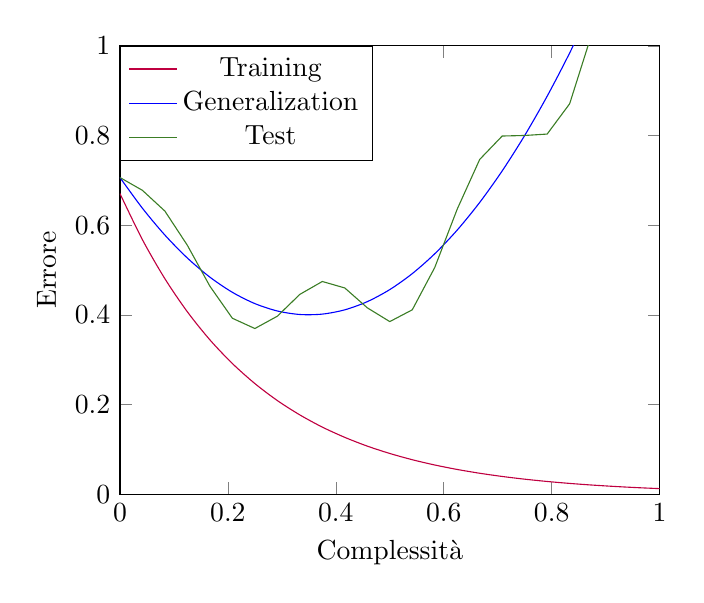
\begin{tikzpicture}
    \begin{axis}[
        ymin=0,ymax=1,
        xmin=0, xmax=1,
        xlabel={Complessità},
        ylabel={Errore},
        legend style={at={(axis cs:0,1)}, anchor=north west}
    ]
    \addplot[smooth, domain=0:1, purple]
        {exp(-4*(x+0.1))}node[pos=1](f1){};
    \addplot[smooth, domain=0:1, blue]
        {2.5*(x-0.35)^2+0.4}node[pos=1](f2){};
    \addplot[domain=0:1, OliveGreen]
        {2.5*(x-0.35)^2+0.4+0.05*sin(1200*x)*exp(x)}node[pos=1](f3){};
    \legend{Training, Generalization, Test};
    \end{axis}
\end{tikzpicture}
\end{document}